\chapter{Metodología} % Main chapter title
\label{Chapter2} % For referencing the chapter elsewhere, use \ref{Chapter1} 

\section{Metodología utilizada}

En el presente proyecto se ha utilizado la metología CRISP DM\parencite{CrispBook1}, pero sólo en las etapas iniciales que tienen que ver con el trabajo de los datos. En la imagen~\ref{fig:crispdm} se pueden ver resaltadas las etapas cubiertas.

\begin{figure}[th]
\centering
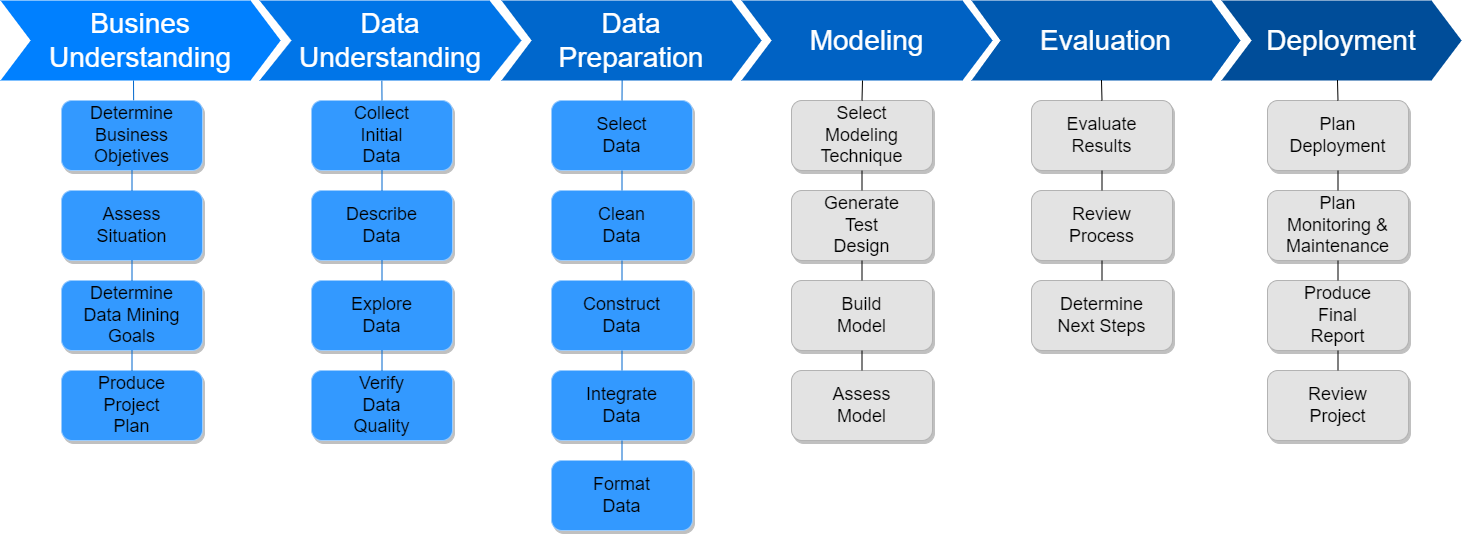
\includegraphics[width=1.2\textwidth]{Figures/modelo_crisp}
\decoRule
\caption[Metodolofía Crisp DM]{Secciones cubiertas en el proyecto}
\label{fig:crispdm}
\end{figure}

\section{Herramientas usadas}

Se han hecho uso de las siguientes herramientas:

\begin{itemize}
\item Base de datos MySql
\item Servicio RDS de AWS
\item R Studio
\item JetBrains DataGrip
\item Shiny
\item Git (github)
\end{itemize}

Se obtuvo un archivo CSV con toda la información de estudiantes, este archivo fue subido mediante DataGrip a una BD MySQL, previamente creada como un servicio RDS de AWS, con estos datos cargados se realizaron procesos mediante R para obtener información que posteriormente fueron registrados en otra base de datos y mostrados mediante una aplicación Shiny.

En la imagen~\ref{fig:proceso} se puede ver el flujo del proceso en este trabajo de análisis.
\begin{figure}[th]
\centering
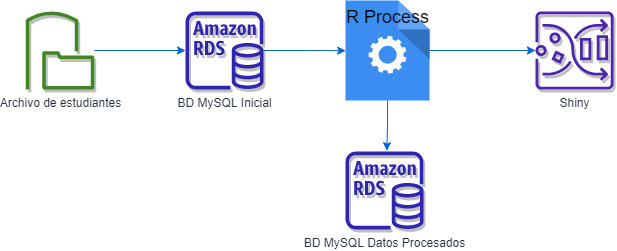
\includegraphics[width=1.1\textwidth]{Figures/proceso-archi}
\decoRule
\caption[Proceso de exploración de los datos]{Herramientas usadas}
\label{fig:proceso}
\end{figure}

\section{Trabajo con los datos}

Para el trabajo con R y MySQL se hizo uso de la bilbioteca RMySQL y DBI, el código para la conexión se encuentra en la sección \ref{codigo_conexionbd}.

\section{Análisis realizados}

\subsection{Niveles educativos}
Para el caso del nivel educativo, es importante conocer la cantidad de alumnos por año en cada nivel, de esta forma identificamos si existe algún incremento o alguna disminución, para lo que se deberá realizar diversas acciones contrarrestando cualquier inconveniente de materiales y de inmobiliarios. \\
En el apéndice \ref{cod_niveles_educativos} está el código fuente de esto.

\subsection{Evolución mensual de matrículas}
\begin{itemize}
\item Se hizo una consulta a la Base de Datos donde se encuentra la tabla estudiante.
\item Debido que sólo había una columna con la fecha de la matrícula en formato YYYY-MM-DD, se obtuvo sólo los valores de año y mes para que se puedan agrupar por este campo.
\item Luego se agrupó esta información por el nuevo campo que contiene el año y el mes.
\item Se categorizó el campo mes.
\item Se agregó un campo de año para que pueda ser filtrado posteriormente.
\end{itemize}

El código para obtener la información para este análisis se encuentra en el anexo \ref{cod_evolucion_matriculas}.

El resultado de este análisis se encuentra en la sección \ref{res_evolucion_matriculas}.

\subsection{Discapacidad}

Para el procesamiento de la data se realizó limpieza de datos vacíos, posterior a eso se agrupó y realizó el conteo de estudiantes que tengan alguna discapacidad.\\
Con estos datos se puede posteriormente filtrar por año para que pueda ser visualizada dinámicamente en shiny. En el apéndice \ref{cod_discapacidad} está el código fuente de esto.

\subsection{Nacionalidades}

Se desea mostrar la cantidad de estudiantes de nacionalidad diferente a la peruana.\\
Para el procesamiento de los datos no se toma en cuenta a los estudiantes con nacionalidad peruana y datos en blanco.\\
En el apéndice \ref{cod_nacionalidades} está el código fuente de esto.

\subsection{Género}

\begin{itemize}
    \item Se analizo la distribución del género de los estudiantes por año, para esto necesitamos todos los DNIs válidos para proceder con el conteo, por lo cual se realizó una limpieza a la data.
    \begin{itemize}
        \item Limpieza a los strings de genero ya que se encontraban con saltos de línea:
        \begin{figure}[th]
        \centering
        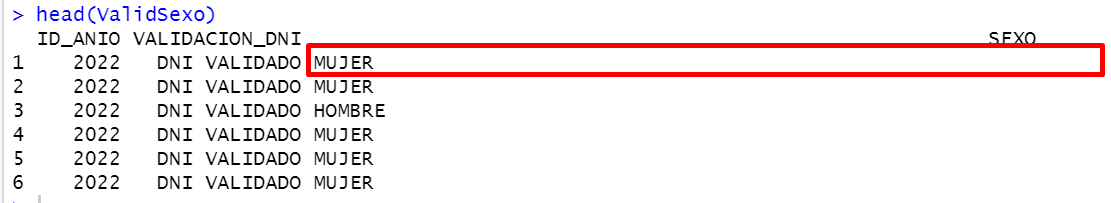
\includegraphics[width=1\textwidth]{Figures/genero1}
        \decoRule
        \caption[]{}
        \label{fig:genero1}
        \end{figure}
        \item Para ello solo extraemos una parte del string (6 primeros caracteres) y está solucionado:
        \begin{figure}[th]
        \centering
        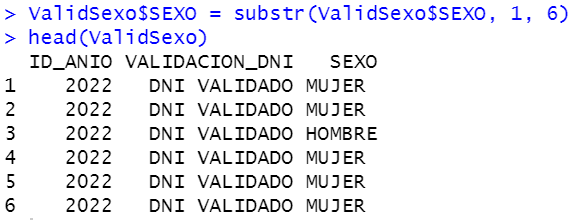
\includegraphics[width=0.6\textwidth]{Figures/genero2}
        \decoRule
        \caption[]{}
        \label{fig:genero2}
        \end{figure}
    \end{itemize}
    \item Se lee la información con un parámetro que quita los registros en blanco, para evitar DNIs que no sean válidos.
\end{itemize}

El código se encuentra en el apéndice \ref{cod_genero}

\subsection{DNI Validados}

\begin{itemize}
    \item Se agrupa el dataframa de estudiantes por el campo de validación de DNI.
    \item Se crea un nuevo DF que contiene el conteo del campo que representa la validación de un DNI.
    \item Se obtiene un porcentaje de los calores del paso anterior.
\end{itemize}

El código se encuentra en el apéndice \ref{cod_dnivalidados}

\section{Uso de shiny}

Se usó Shiny \parencite{ShinyRef} para mostrar los análisis de manera interactiva, ya que se tiene información de 3 años (2020, 2021 y 2022). 

Los componentes utilizados en el proyecto fueron tablas, gráfico de barras, gráfico circular y gráfico de líneas \parencite{RBook1}.
El código para realizar esta funcionalidad se encuentra en el anexo \ref{cod_shiny}.

Para la publicación se hace uso del servidor que brinda RStudio \parencite{ShinyAppRef}.
 
\section{Fuentes}
Las fuentes del proyecto se encuentran en el repositorio Git: \url{https://github.com/Maestria-Data-Science-UPC-G1/gestiondatos.git}